% this template would fit in 16:9 ratio
% if you wanna use 4:3, you have to fix the package
\documentclass[aspectratio=169]{beamer}

% the theme UM498 defined in the .sty file
\usetheme{UM498}

% show page number, as required by the spec...
\setbeamertemplate{footline}[page number]{}
%gets rid of navigation symbols, no authors, title, etc at the foot. (Because too many authors will be shown...)
\setbeamertemplate{navigation symbols}{}

%\setbeameroption{show notes}
%\setbeameroption{show only notes}
\setbeamerfont{note page}{size=\fontsize{0.2cm}{0.1cm}}

\usepackage{media9,tagging}
\usepackage{pgfplots}
\usepackage{amsmath}
\pgfplotsset{compat=1.10}
\usetikzlibrary{calc}
\usepackage[utf8]{inputenc}
\usepackage[T1]{fontenc}

\usepackage{helvet,multicol}
\newcommand\Newline{\newline\newline}

\title{Conversational Yelp}

% \subtitle{Subtitle}
\author{Binqi Sun, Fanhao Zeng, Jiangchen Zhu, Qichen Fu, Yiming Shi, Yongwei Yuan, Yujian Liu, Yuhang Zhou}
\date{January 29, 2020}
\institute{\{sbq, zfh, zjcsjtu, fuqichen, syiming, slark, yujianl, tonyzhou\}@umich.edu}

\begin{document}

% welcome page
\begin{frame}[plain,t]
\titlepage
\end{frame}


\section{Problem Statement}
\begin{frame}{Problem Statement}
\begin{columns}
    \begin{column}{8cm}
        \begin{figure}
        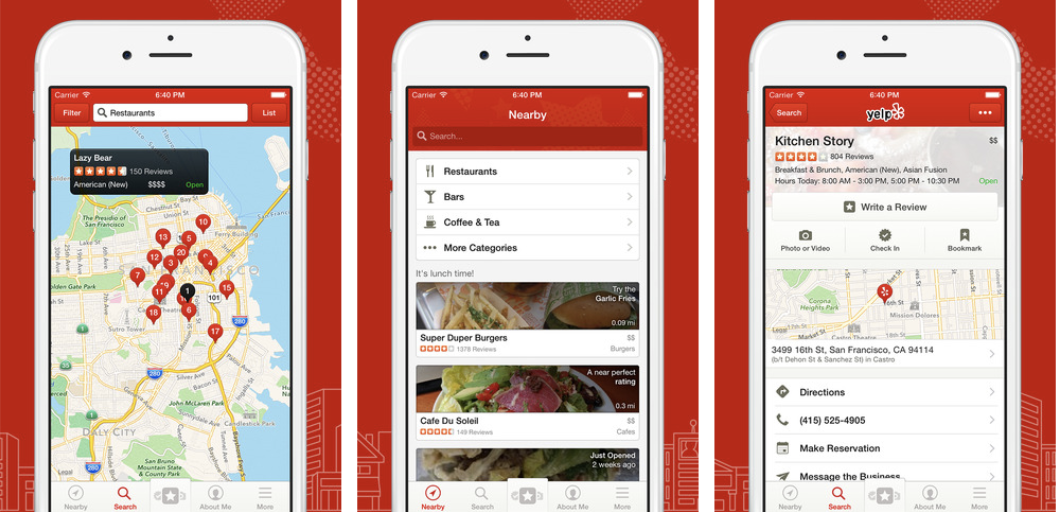
\includegraphics[width=8cm]{image1}
        \end{figure}
    \end{column}
    \pause
    \begin{column}{2.5cm}
        \begin{figure}
        
\includegraphics[width=2.5cm]{image2}
        \end{figure}
    \end{column}
\end{columns}
\vspace{1em}
\begin{enumerate}
    \item Too complicated
    \item Not accessible to all people
\end{enumerate}
\end{frame}

% \subsection{Subsection}

\section{Conversational Restaurant Recommendation}
\begin{frame}{Conversational Restaurant Recommendation}
    \begin{enumerate}
        \item Price, location, cuisine, popularity
        \item Open time
        \item Seat reservation, estimated available time
        \item Drive-through
    \end{enumerate}
\end{frame}

\section{Project Description}
\begin{frame}{Project Description}
\textbf{You can ask:}
\begin{enumerate}
        \item Show me some well-rated restaurants near me
        \item I want to have dinner with my girlfriend at 6 pm
\end{enumerate}
\pause
\vspace{2em}
\textbf{We can remember your preference:}
\begin{enumerate}
    \item That’s too expensive
    \item I don’t like noodles

\end{enumerate}
\end{frame}


\section{Architecture}
\begin{frame}{Architecture}
\begin{figure}
        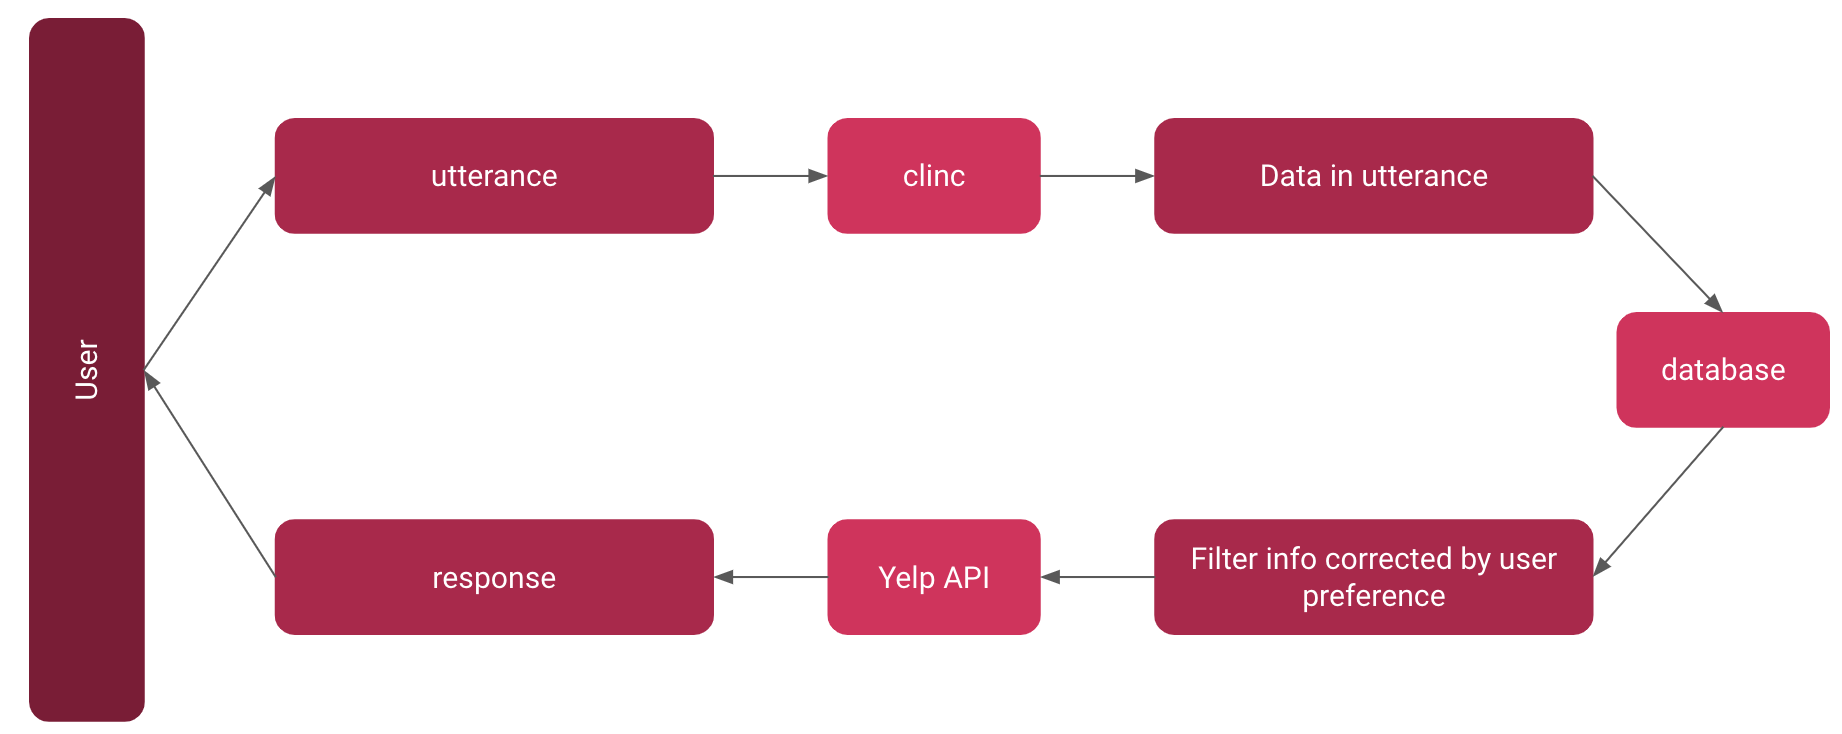
\includegraphics[width=13cm]{image3}
\end{figure}
\end{frame}

\section{Success Milestones}
\begin{frame}{Success Milestones}
\begin{figure}
        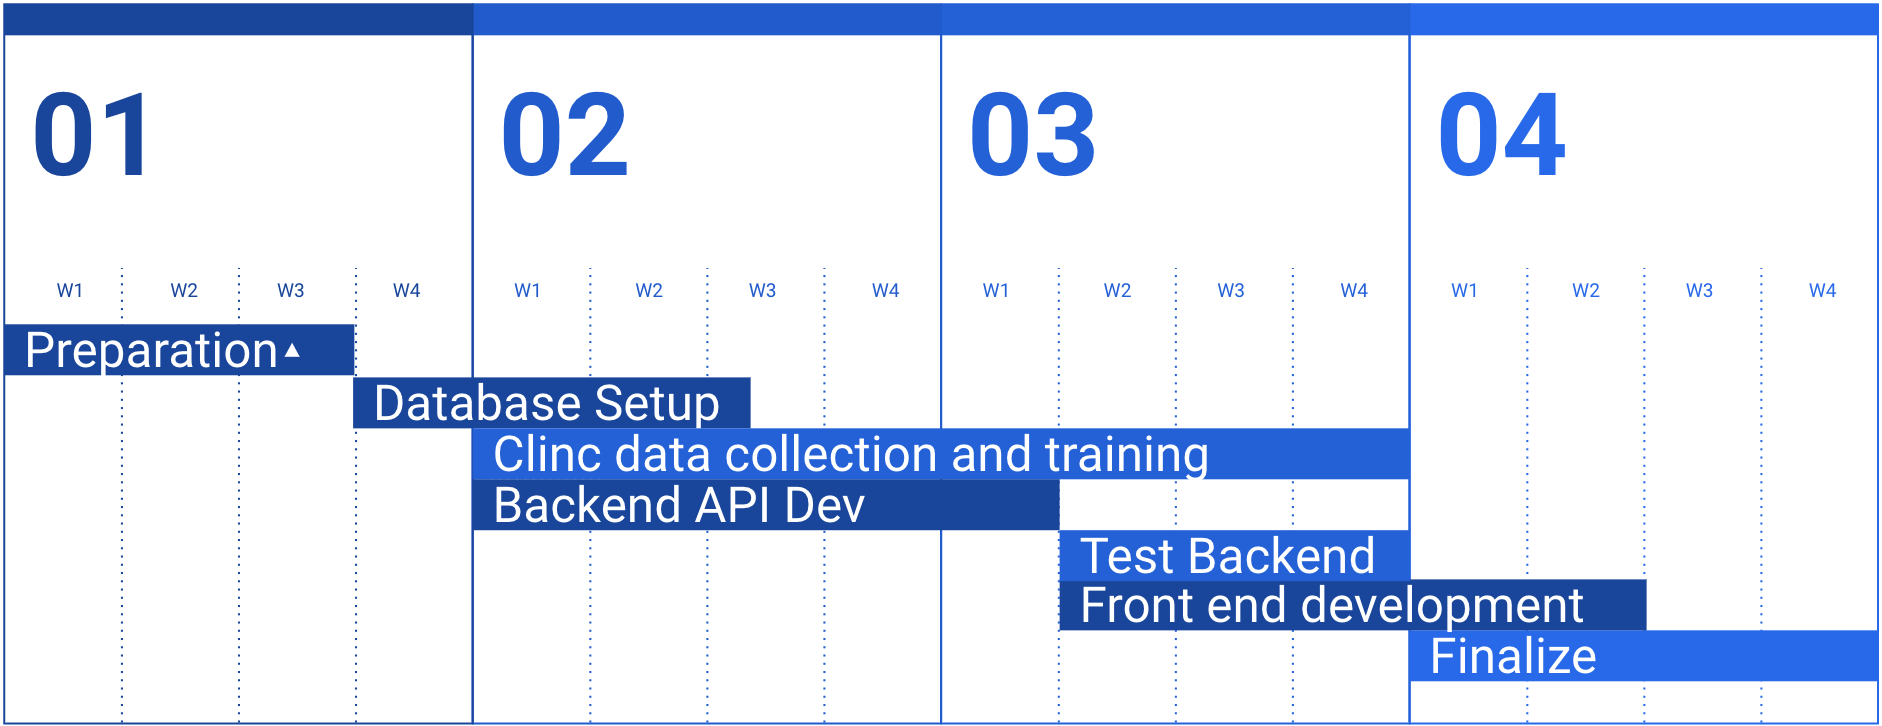
\includegraphics[width=13cm]{image4}
\end{figure}
\end{frame}

\section{Related Technologies}
\begin{frame}{Related Technologies}
\begin{enumerate}
    \item Google Speech-to-Text, voice recognition
\item Clinc stack, data extraction
\item Mongodb, store user preference
\item Yelp API, query restaurant information

\end{enumerate}
\end{frame}

\section{Summary}
\begin{frame}{Summary}
\begin{figure}
        
\includegraphics[width=10cm]{image5}
\end{figure}

\end{frame}

% \section{References}
% \begin{frame}[allowframebreaks]{References}

% \end{frame}

% thank-you frame defined by theme UM498.
\ThankYouFrame

\end{document}